\documentclass[11pt]{article}

% Mandatory Packages
\usepackage{amsmath}
\usepackage{amssymb}
\usepackage{amsthm}
\usepackage{geometry}
\usepackage{tikz}
\usetikzlibrary{arrows.meta, positioning, shapes, calc}
\usepackage{mathrsfs}
\usepackage{mathtools}
\usepackage{hyperref}

% Page Geometry
\geometry{letterpaper, margin=1in}

% Theorem Environments
\newtheorem{theorem}{Theorem}[section]
\newtheorem{lemma}[theorem]{Lemma}
\newtheorem{proposition}[theorem]{Proposition}
\newtheorem{corollary}[theorem]{Corollary}
\newtheorem{definition}{Definition}[section]
\newtheorem{problem}{Problem}
\newtheorem{flaw}{Flawed Proof}

% Custom Commands
\newcommand{\Z}{\mathbb{Z}}
\newcommand{\R}{\mathbb{R}}
\newcommand{\N}{\mathbb{N}}
\newcommand{\Q}{\mathbb{Q}}
\newcommand{\modulo}[1]{\ (\mathrm{mod}\ #1)}

\title{\textbf{Homework 4 Proofs Involving Congruence of Integers}}
\author{Tashfeen Omran}
\date{September 2026}

\begin{document}

\maketitle
\tableofcontents
\newpage

% ==========================================
% PART 1: Comprehensive Introduction
% ==========================================
\section{Part 1: Comprehensive Introduction, Context, and Prerequisites}

\subsection{Core Concepts \& Axioms}
In the realm of abstract mathematics, the concept of equality is often too restrictive. We frequently encounter scenarios where distinct objects behave identically under a specific structural lens. In number theory and algebra, this is formalized through \textbf{congruence}. 

\begin{definition}[Congruence Modulo $n$]
Let $a, b \in \Z$ and let $n \in \Z$ such that $n \geq 2$. We say that $a$ is congruent to $b$ modulo $n$, written as $a \equiv b \modulo{n}$, if and only if $n$ divides the difference $(a - b)$. Formally:
\[ a \equiv b \modulo{n} \iff n \mid (a - b) \iff \exists k \in \Z \text{ such that } a - b = kn \]
\end{definition}

This definition introduces an \textbf{equivalence relation} on the set of integers, $\Z$. An equivalence relation partitions a set into disjoint subsets called \textbf{equivalence classes} (or residue classes). For a given modulus $n$, there are exactly $n$ distinct equivalence classes, typically represented by the remainders $\{0, 1, \dots, n-1\}$.

\subsection{Intuition and Set-Theoretic Foundations}
To understand the "why" behind congruence, imagine a mapping from the infinite space of integers $\Z$ to a finite, circular space. The classic intuition is "clock arithmetic." On a standard 12-hour clock, 13:00 and 1:00 represent the same position. Set-theoretically, we are defining a quotient space, denoted as $\Z/n\Z$. 

When we write $a \equiv b \modulo{n}$, we are asserting that $a$ and $b$ belong to the exact same partition in $\Z/n\Z$. Because they belong to the same partition, they are algebraically indistinguishable under addition and multiplication within this modular space. This allows us to reduce infinitely large integers to manageable, finite representatives without losing structural integrity.

\subsection{Historical Context and Motivation}
The formalization of modular arithmetic was introduced by the legendary mathematician Carl Friedrich Gauss in his seminal 1801 work, \textit{Disquisitiones Arithmeticae}. Before Gauss, mathematicians studied divisibility on an ad-hoc basis. Gauss recognized that by treating "having the same remainder" as a form of equality, he could port the powerful tools of standard algebra (equations, polynomials) into the discrete world of number theory. This paradigm shift laid the groundwork for modern abstract algebra, cryptography, and computer science.

\subsection{Key Theorems, Lemmas, and Formulas}
\begin{theorem}[Properties of Congruence]
Let $a, b, c, d \in \Z$ and $n \geq 2$. If $a \equiv b \modulo{n}$ and $c \equiv d \modulo{n}$, then:
\begin{enumerate}
    \item \textbf{Addition:} $a + c \equiv b + d \modulo{n}$
    \item \textbf{Multiplication:} $ac \equiv bd \modulo{n}$
    \item \textbf{Exponentiation:} $a^k \equiv b^k \modulo{n}$ for any integer $k \geq 1$.
\end{enumerate}
\end{theorem}

\begin{theorem}[Equivalence Relation Properties]
Congruence modulo $n$ is an equivalence relation on $\Z$:
\begin{enumerate}
    \item \textbf{Reflexive:} $a \equiv a \modulo{n}$
    \item \textbf{Symmetric:} If $a \equiv b \modulo{n}$, then $b \equiv a \modulo{n}$
    \item \textbf{Transitive:} If $a \equiv b \modulo{n}$ and $b \equiv c \modulo{n}$, then $a \equiv c \modulo{n}$
\end{enumerate}
\end{theorem}

\subsection{Prerequisites}
To master this chapter, you must be fluent in:
\begin{itemize}
    \item \textbf{Divisibility Definition:} $a \mid b \iff b = ak$ for some $k \in \Z$.
    \item \textbf{Direct Proofs:} Assuming $P$ to logically deduce $Q$.
    \item \textbf{Proof by Cases (Exhaustion):} Utilizing the Division Algorithm to partition integers into forms like $3q, 3q+1, 3q+2$.
    \item \textbf{Basic Algebraic Expansion:} Expanding polynomials like $(x+y)^2$ and $(x+y)^3$.
\end{itemize}

\newpage
% ==========================================
% PART 2: Detailed Homework Solutions
% ==========================================
\section{Part 2: Detailed Homework Solutions}
\textit{Note: Based on strategic problem selection, the following problems cover every distinct archetype present in Section 4.2, ensuring comprehensive mastery without redundant repetition.}

\begin{problem}[Exercise 4.14]
Let $a, b, n \in \Z$, where $n \geq 2$. Prove that if $a \equiv b \modulo{n}$, then $a^2 \equiv b^2 \modulo{n}$.
\end{problem}
\begin{proof}
\textbf{Proof Technique:} Direct Proof. \\
\textbf{Assumptions:} Assume $a \equiv b \modulo{n}$. \\
By the definition of congruence, $a \equiv b \modulo{n}$ implies that $n \mid (a - b)$. 
By the definition of divisibility, there exists an integer $k$ such that:
\[ a - b = nk \]
We wish to show that $a^2 \equiv b^2 \modulo{n}$, which means we must show $n \mid (a^2 - b^2)$.
Consider the expression $a^2 - b^2$. By the difference of squares factorization, we have:
\[ a^2 - b^2 = (a - b)(a + b) \]
Substitute $a - b = nk$ into the equation:
\[ a^2 - b^2 = (nk)(a + b) = n(k(a + b)) \]
Since $k, a, b \in \Z$, the set of integers is closed under addition and multiplication, meaning $k(a + b)$ is an integer. Let $m = k(a + b)$, where $m \in \Z$.
Thus, we have:
\[ a^2 - b^2 = nm \]
By the definition of divisibility, this implies $n \mid (a^2 - b^2)$. 
Therefore, by the definition of congruence, $a^2 \equiv b^2 \modulo{n}$.
\end{proof}

\vspace{0.5cm}

\begin{problem}[Exercise 4.15]
Let $a, b, c, n \in \Z$, where $n \geq 2$. Prove that if $a \equiv b \modulo{n}$ and $b \equiv c \modulo{n}$, then $a \equiv c \modulo{n}$.
\end{problem}
\begin{proof}
\textbf{Proof Technique:} Direct Proof (establishing Transitivity). \\
\textbf{Assumptions:} Assume $a \equiv b \modulo{n}$ and $b \equiv c \modulo{n}$. \\
By the definition of congruence, these assumptions imply:
\[ n \mid (a - b) \quad \text{and} \quad n \mid (b - c) \]
By the definition of divisibility, there exist integers $k, j \in \Z$ such that:
\[ a - b = nk \]
\[ b - c = nj \]
We wish to show that $a \equiv c \modulo{n}$, which requires showing $n \mid (a - c)$.
Consider the expression $a - c$. We can rewrite this by adding and subtracting $b$:
\[ a - c = a - b + b - c \]
Substitute the expressions for $(a - b)$ and $(b - c)$:
\[ a - c = nk + nj \]
Factor out the common term $n$:
\[ a - c = n(k + j) \]
Since $k, j \in \Z$, their sum $k + j$ is also an integer. Let $m = k + j$, where $m \in \Z$.
Thus, $a - c = nm$. By the definition of divisibility, $n \mid (a - c)$.
Therefore, $a \equiv c \modulo{n}$.
\end{proof}

\vspace{0.5cm}

\begin{problem}[Exercise 4.16]
Let $a, b \in \Z$. Prove that $a^2 + 2b^2 \equiv 0 \modulo{3}$ if and only if either $a$ and $b$ are both congruent to $0$ modulo $3$ or neither is congruent to $0$ modulo $3$.
\end{problem}
\begin{proof}
\textbf{Proof Technique:} Biconditional Proof using Proof by Cases (Exhaustion). \\
First, we establish a lemma regarding squares modulo 3. By the Division Algorithm, any integer $x$ is congruent to $0, 1,$ or $2 \modulo{3}$.
\begin{itemize}
    \item If $x \equiv 0 \modulo{3}$, then $x^2 \equiv 0^2 \equiv 0 \modulo{3}$.
    \item If $x \equiv 1 \modulo{3}$, then $x^2 \equiv 1^2 \equiv 1 \modulo{3}$.
    \item If $x \equiv 2 \modulo{3}$, then $x^2 \equiv 2^2 = 4 \equiv 1 \modulo{3}$.
\end{itemize}
Thus, for any integer $x$, $x^2 \equiv 0 \modulo{3}$ (if $x \equiv 0 \modulo{3}$) or $x^2 \equiv 1 \modulo{3}$ (if $x \not\equiv 0 \modulo{3}$).

\textbf{Part 1: ($\impliedby$)} Assume either ($a \equiv 0 \modulo{3}$ and $b \equiv 0 \modulo{3}$) OR ($a \not\equiv 0 \modulo{3}$ and $b \not\equiv 0 \modulo{3}$).
\textit{Case 1:} $a \equiv 0 \modulo{3}$ and $b \equiv 0 \modulo{3}$.
Then $a^2 \equiv 0 \modulo{3}$ and $b^2 \equiv 0 \modulo{3}$.
\[ a^2 + 2b^2 \equiv 0 + 2(0) \equiv 0 \modulo{3} \]
\textit{Case 2:} $a \not\equiv 0 \modulo{3}$ and $b \not\equiv 0 \modulo{3}$.
From our lemma, $a^2 \equiv 1 \modulo{3}$ and $b^2 \equiv 1 \modulo{3}$.
\[ a^2 + 2b^2 \equiv 1 + 2(1) = 3 \equiv 0 \modulo{3} \]
In both cases, $a^2 + 2b^2 \equiv 0 \modulo{3}$.

\textbf{Part 2: ($\implies$)} We prove the contrapositive: If it is NOT the case that (both are $0 \modulo{3}$ or neither is $0 \modulo{3}$), then $a^2 + 2b^2 \not\equiv 0 \modulo{3}$.
The negation of the hypothesis is that exactly one of $a$ or $b$ is congruent to $0 \modulo{3}$.
\textit{Case 1:} $a \equiv 0 \modulo{3}$ and $b \not\equiv 0 \modulo{3}$.
Then $a^2 \equiv 0 \modulo{3}$ and $b^2 \equiv 1 \modulo{3}$.
\[ a^2 + 2b^2 \equiv 0 + 2(1) = 2 \not\equiv 0 \modulo{3} \]
\textit{Case 2:} $a \not\equiv 0 \modulo{3}$ and $b \equiv 0 \modulo{3}$.
Then $a^2 \equiv 1 \modulo{3}$ and $b^2 \equiv 0 \modulo{3}$.
\[ a^2 + 2b^2 \equiv 1 + 2(0) = 1 \not\equiv 0 \modulo{3} \]
In both cases, $a^2 + 2b^2 \not\equiv 0 \modulo{3}$. By contrapositive, the forward direction holds.
Since both directions hold, the biconditional is proven.
\end{proof}

\vspace{0.5cm}

\begin{problem}[Exercise 4.18]
Let $m, n \in \N$ such that $m \mid n$. Prove that if $a$ and $b$ are integers such that $a \equiv b \modulo{n}$, then $a \equiv b \modulo{m}$.
\end{problem}
\begin{proof}
\textbf{Proof Technique:} Direct Proof. \\
\textbf{Assumptions:} Assume $m \mid n$ and $a \equiv b \modulo{n}$. \\
By the definition of divisibility, $m \mid n$ implies there exists an integer $k$ such that:
\[ n = mk \]
By the definition of congruence, $a \equiv b \modulo{n}$ implies $n \mid (a - b)$. Thus, there exists an integer $j$ such that:
\[ a - b = nj \]
We wish to show that $a \equiv b \modulo{m}$, which means we must show $m \mid (a - b)$.
Substitute the expression $n = mk$ into the equation for $a - b$:
\[ a - b = (mk)j = m(kj) \]
Since $k, j \in \Z$, their product $kj$ is an integer. Let $q = kj$, where $q \in \Z$.
Thus, $a - b = mq$. By the definition of divisibility, this implies $m \mid (a - b)$.
Therefore, $a \equiv b \modulo{m}$.
\end{proof}

\vspace{0.5cm}

\begin{problem}[Exercise 4.19]
Let $a, b \in \Z$. Show that if $a \equiv 5 \modulo{6}$ and $b \equiv 3 \modulo{4}$, then $4a + 6b \equiv 6 \modulo{8}$.
\end{problem}
\begin{proof}
\textbf{Proof Technique:} Direct Proof via Algebraic Substitution. \\
\textbf{Assumptions:} Assume $a \equiv 5 \modulo{6}$ and $b \equiv 3 \modulo{4}$. \\
By the definition of congruence, there exist integers $k, j \in \Z$ such that:
\[ a - 5 = 6k \implies a = 6k + 5 \]
\[ b - 3 = 4j \implies b = 4j + 3 \]
We wish to evaluate the expression $4a + 6b$ modulo 8. Substitute the expressions for $a$ and $b$:
\[ 4a + 6b = 4(6k + 5) + 6(4j + 3) \]
Distribute the constants:
\[ 4a + 6b = 24k + 20 + 24j + 18 \]
Combine like terms:
\[ 4a + 6b = 24k + 24j + 38 \]
We want to show this is congruent to $6 \modulo{8}$. We can rewrite 38 as $32 + 6$:
\[ 4a + 6b = 24k + 24j + 32 + 6 \]
Factor out an 8 from the first three terms:
\[ 4a + 6b = 8(3k + 3j + 4) + 6 \]
Let $m = 3k + 3j + 4$. Since $k, j \in \Z$, $m \in \Z$.
\[ 4a + 6b = 8m + 6 \]
Subtract 6 from both sides:
\[ (4a + 6b) - 6 = 8m \]
By the definition of divisibility, $8 \mid ((4a + 6b) - 6)$.
Therefore, $4a + 6b \equiv 6 \modulo{8}$.
\end{proof}

\vspace{0.5cm}

\begin{problem}[Exercise 4.21]
Let $a \in \Z$. Prove that $a^3 \equiv a \modulo{3}$.
\end{problem}
\begin{proof}
\textbf{Proof Technique:} Proof by Cases (Exhaustion). \\
By the Division Algorithm, any integer $a$ must be congruent to exactly one of $0, 1,$ or $2$ modulo $3$. We examine each case.

\textit{Case 1:} $a \equiv 0 \modulo{3}$.
Then $a^3 \equiv 0^3 = 0 \modulo{3}$.
Thus, $a^3 \equiv a \modulo{3}$ holds ($0 \equiv 0 \modulo{3}$).

\textit{Case 2:} $a \equiv 1 \modulo{3}$.
Then $a^3 \equiv 1^3 = 1 \modulo{3}$.
Thus, $a^3 \equiv a \modulo{3}$ holds ($1 \equiv 1 \modulo{3}$).

\textit{Case 3:} $a \equiv 2 \modulo{3}$.
Then $a^3 \equiv 2^3 = 8 \modulo{3}$.
Since $8 = 3(2) + 2$, we have $8 \equiv 2 \modulo{3}$.
Thus, $a^3 \equiv 2 \equiv a \modulo{3}$.

In all possible cases, $a^3 \equiv a \modulo{3}$.
\end{proof}

\vspace{0.5cm}

\begin{problem}[Exercise 4.24]
Let $x$ and $y$ be even integers. Prove that $x^2 \equiv y^2 \modulo{16}$ if and only if either (a) $x \equiv 0 \modulo{4}$ and $y \equiv 0 \modulo{4}$ or (b) $x \equiv 2 \modulo{4}$ and $y \equiv 2 \modulo{4}$.
\end{problem}
\begin{proof}
\textbf{Proof Technique:} Biconditional Proof. \\
Since $x$ and $y$ are even integers, there exist integers $a, b \in \Z$ such that $x = 2a$ and $y = 2b$.
Substitute these into the congruence $x^2 \equiv y^2 \modulo{16}$:
\[ (2a)^2 \equiv (2b)^2 \modulo{16} \iff 4a^2 \equiv 4b^2 \modulo{16} \]
By definition, this means $16 \mid (4a^2 - 4b^2)$, which simplifies to $16 \mid 4(a^2 - b^2)$.
Dividing by 4, this is equivalent to $4 \mid (a^2 - b^2)$, which means:
\[ a^2 \equiv b^2 \modulo{4} \]
We know that for any integer $k$, $k^2 \equiv 0 \modulo{4}$ if $k$ is even, and $k^2 \equiv 1 \modulo{4}$ if $k$ is odd.
Therefore, $a^2 \equiv b^2 \modulo{4}$ if and only if $a$ and $b$ have the same parity (both even or both odd).

\textbf{Part 1: ($\impliedby$)} Assume (a) or (b) holds.
If (a) holds, $x \equiv 0 \modulo{4}$ and $y \equiv 0 \modulo{4}$. Then $x = 4k$ and $y = 4j$.
$x^2 = 16k^2 \equiv 0 \modulo{16}$ and $y^2 = 16j^2 \equiv 0 \modulo{16}$. Thus $x^2 \equiv y^2 \modulo{16}$.
If (b) holds, $x \equiv 2 \modulo{4}$ and $y \equiv 2 \modulo{4}$. Then $x = 4k+2$ and $y = 4j+2$.
$x^2 = 16k^2 + 16k + 4 \equiv 4 \modulo{16}$.
$y^2 = 16j^2 + 16j + 4 \equiv 4 \modulo{16}$.
Thus $x^2 \equiv y^2 \modulo{16}$.

\textbf{Part 2: ($\implies$)} Assume $x^2 \equiv y^2 \modulo{16}$.
As shown above, this implies $a$ and $b$ have the same parity, where $x=2a$ and $y=2b$.
\textit{Case 1:} $a$ and $b$ are both even. Let $a = 2k$ and $b = 2j$.
Then $x = 2(2k) = 4k \implies x \equiv 0 \modulo{4}$.
And $y = 2(2j) = 4j \implies y \equiv 0 \modulo{4}$. This is condition (a).
\textit{Case 2:} $a$ and $b$ are both odd. Let $a = 2k+1$ and $b = 2j+1$.
Then $x = 2(2k+1) = 4k+2 \implies x \equiv 2 \modulo{4}$.
And $y = 2(2j+1) = 4j+2 \implies y \equiv 2 \modulo{4}$. This is condition (b).
Thus, $x^2 \equiv y^2 \modulo{16}$ implies either (a) or (b) must be true.
\end{proof}

\newpage
% ==========================================
% PART 3: In-Depth Analysis
% ==========================================
\section{Part 3: In-Depth Analysis of Problems and Techniques}

\subsection{A) Problem Types and Logical Strategies}
The problems in this section fall into three distinct archetypes:
\begin{enumerate}
    \item \textbf{Direct Algebraic Manipulation (e.g., 4.14, 4.15, 4.18, 4.19):} 
    \textit{Strategy:} Unpack the definition of congruence into its divisibility form ($a - b = nk$). Perform standard algebraic operations (substitution, factoring, distribution) on the integers, and then repackage the result back into a congruence statement.
    \item \textbf{Exhaustive Residue Checking / Proof by Cases (e.g., 4.16, 4.21):}
    \textit{Strategy:} When the modulus $n$ is small (like 3 or 4), the most efficient strategy is to partition the integers into $n$ equivalence classes. By testing the property on the finite set of representatives $\{0, 1, \dots, n-1\}$, you prove the property holds for all integers.
    \item \textbf{Biconditional Parity and Modulus Reduction (e.g., 4.24):}
    \textit{Strategy:} For "if and only if" statements involving squares and larger moduli (like 16), it is often necessary to divide out common factors from the modulus (reducing modulo 16 to modulo 4) to reveal underlying parity constraints.
\end{enumerate}

\subsection{B) Key Analytical and Logical Manipulations}
\begin{itemize}
    \item \textbf{Difference of Squares Factorization:} Used in 4.14. $a^2 - b^2 = (a-b)(a+b)$. Because congruence implies $n \mid (a-b)$, it trivially divides any multiple of $(a-b)$.
    \item \textbf{Adding Zero / Telescoping:} Used in 4.15. To bridge $a$ to $c$, we write $a - c = (a - b) + (b - c)$. This is a fundamental trick in analysis (e.g., Triangle Inequality proofs) adapted for discrete divisibility.
    \item \textbf{Contrapositive for "OR" Statements:} In 4.16, proving the forward direction of a biconditional where the conclusion is an "OR" statement is difficult directly. Using the contrapositive allows us to negate the "OR" into an "AND" (De Morgan's Laws), providing concrete cases to test.
    \item \textbf{Modulus Factoring:} In 4.24, translating $16 \mid 4(a^2 - b^2)$ to $4 \mid (a^2 - b^2)$ is a crucial algebraic step. It relies on the theorem that if $kn \mid km$, then $n \mid m$.
\end{itemize}

\newpage
% ==========================================
% PART 4: Cheatsheet, Visuals, and Tips
% ==========================================
\section{Part 4: "Cheatsheet", Visuals, and Tips for Success}

\subsection{Theorems \& Equivalences}
\begin{itemize}
    \item \textbf{Definition:} $a \equiv b \modulo{n} \iff n \mid (a-b) \iff a = b + kn$.
    \item \textbf{Addition/Subtraction:} $a \equiv b \implies a \pm c \equiv b \pm c \modulo{n}$.
    \item \textbf{Multiplication:} $a \equiv b \implies ac \equiv bc \modulo{n}$.
    \item \textbf{Powers:} $a \equiv b \implies a^k \equiv b^k \modulo{n}$ for $k \in \N$.
    \item \textbf{Polynomials:} If $P(x)$ is a polynomial with integer coefficients, $a \equiv b \modulo{n} \implies P(a) \equiv P(b) \modulo{n}$.
\end{itemize}

\subsection{Set \& Logic Illustrations}
The following TikZ diagram illustrates the concept of partitioning $\Z$ into equivalence classes modulo 3. The infinite set of integers is mapped into exactly three distinct residue classes.

\begin{center}
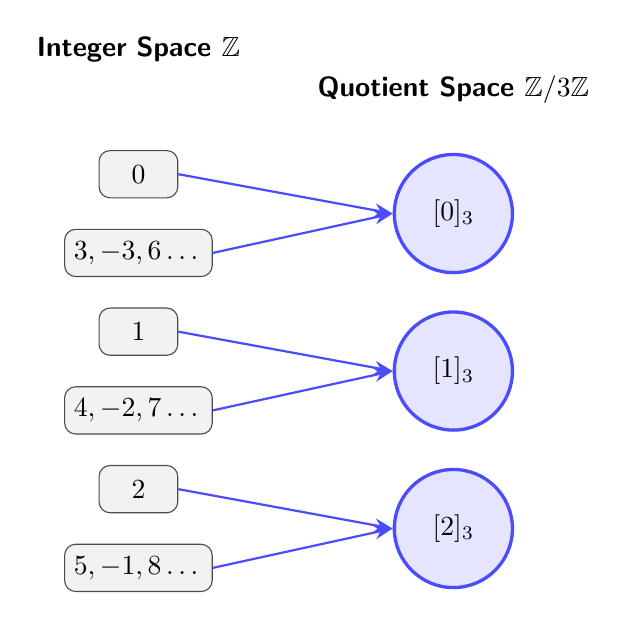
\begin{tikzpicture}[
    >=Stealth,
    node distance=2cm and 4cm,
    every node/.style={font=\sffamily},
    classnode/.style={circle, draw=blue!70, fill=blue!10, very thick, minimum size=1.5cm, align=center},
    intnode/.style={rectangle, draw=black!70, fill=gray!10, rounded corners, minimum width=1cm, minimum height=0.6cm}
]

% Residue Classes
\node[classnode] (c0) at (0, 2) {$[0]_3$};
\node[classnode] (c1) at (0, 0) {$[1]_3$};
\node[classnode] (c2) at (0, -2) {$[2]_3$};

% Integers
\node[intnode] (i0) at (-4, 2.5) {$0$};
\node[intnode] (i3) at (-4, 1.5) {$3, -3, 6 \dots$};

\node[intnode] (i1) at (-4, 0.5) {$1$};
\node[intnode] (i4) at (-4, -0.5) {$4, -2, 7 \dots$};

\node[intnode] (i2) at (-4, -1.5) {$2$};
\node[intnode] (i5) at (-4, -2.5) {$5, -1, 8 \dots$};

% Arrows
\draw[->, thick, blue!70] (i0.east) -- (c0.west);
\draw[->, thick, blue!70] (i3.east) -- (c0.west);

\draw[->, thick, blue!70] (i1.east) -- (c1.west);
\draw[->, thick, blue!70] (i4.east) -- (c1.west);

\draw[->, thick, blue!70] (i2.east) -- (c2.west);
\draw[->, thick, blue!70] (i5.east) -- (c2.west);

% Labels
\node[above=0.5cm of c0] {\textbf{Quotient Space $\Z/3\Z$}};
\node[above=1cm of i0] {\textbf{Integer Space $\Z$}};

\end{tikzpicture}
\end{center}

\subsection{Heuristics \& "Cheats"}
\begin{itemize}
    \item \textbf{The "Small Modulus" Cheat:} If a problem asks you to prove a property for all integers modulo $n$ where $n \leq 5$, immediately use Proof by Cases. It is almost always faster than algebraic manipulation.
    \item \textbf{The "Substitute Early" Rule:} When evaluating complex expressions like $4a + 6b \modulo{8}$, substitute the definition $a = 6k+5$ immediately. Do not try to manipulate the congruences directly if the moduli are different (e.g., mod 6 and mod 4).
\end{itemize}

\subsection{Pitfalls \& Fallacies}
\begin{itemize}
    \item \textbf{The Division Fallacy:} You \textbf{cannot} generally divide congruences. $ac \equiv bc \modulo{n}$ does NOT imply $a \equiv b \modulo{n}$. For example, $2 \cdot 3 \equiv 2 \cdot 0 \modulo{6}$, but $3 \not\equiv 0 \modulo{6}$. Division is only valid if $\gcd(c, n) = 1$.
    \item \textbf{The Exponent Fallacy:} You \textbf{cannot} do arithmetic in the exponent modulo $n$. $2^x \equiv 2^y \modulo{3}$ does NOT mean $x \equiv y \modulo{3}$. (Exponents operate modulo $\phi(n)$, Euler's totient function, not modulo $n$).
\end{itemize}

\newpage
% ==========================================
% PART 5: Conceptual Synthesis
% ==========================================
\section{Part 5: Conceptual Synthesis and The "Big Picture"}

\subsection{A) Thematic Connections}
The core theme of this chapter is \textbf{Equivalence Relations and Quotient Spaces}. By defining congruence, we are formally defining a way to treat distinct objects as "equal" under a specific structural constraint. This unifies previous topics in set theory (partitions) and logic (biconditionals). Just as a probability measure maps a complex sample space $\Omega$ to the interval $[0,1]$, the modulo operator maps the infinite space of integers $\Z$ to a finite, bounded state space $\Z/n\Z$.

\subsection{B) Forward and Backward Links}
\begin{itemize}
    \item \textbf{Backward Links:} This topic relies heavily on the Division Algorithm and the formal definition of divisibility established in earlier chapters. It is the logical culmination of direct proof techniques applied to algebraic structures.
    \item \textbf{Forward Links:} Understanding $\Z/n\Z$ is the absolute bedrock for Abstract Algebra (Groups, Rings, Fields). Furthermore, in advanced probability and stochastic processes, the concept of mapping infinite paths to finite states is mirrored in Markov Chains (state space partitioning) and ergodic theory.
\end{itemize}

% ==========================================
% PART 6: Abstract Real-World Modeling
% ==========================================
\section{Part 6: Abstract Real-World Modeling (AI, ML, \& Quant Finance)}

\subsection{A) Concrete Scenarios}
\begin{enumerate}
    \item \textbf{Algorithmic Trading \& Hash Tables:} High-frequency trading (HFT) systems must process millions of order-book updates per second. To achieve $O(1)$ lookup times for specific stock tickers, HFT systems use Hash Maps. The core of a hash function is modular arithmetic: $h(k) = k \modulo{m}$, ensuring data is uniformly distributed across memory addresses.
    \item \textbf{Cryptography (RSA) in FinTech:} Secure financial transactions rely on RSA encryption, which is entirely built on modular exponentiation and the difficulty of factoring large primes. The theorems of congruence are what allow a bank to decrypt a message that was encrypted with a public key.
    \item \textbf{Monte Carlo Simulations (Quant Finance):} Pricing complex exotic derivatives (like Asian options) requires simulating millions of potential future stock price paths. This requires massive amounts of random numbers. Computers generate these using \textit{Linear Congruential Generators} (LCGs), which rely strictly on congruence relations.
\end{enumerate}

\subsection{B) Model Problem Setup: Linear Congruential Generators for SDEs}
Suppose we are a quantitative researcher pricing a derivative whose underlying asset $S_t$ follows Geometric Brownian Motion, described by the Stochastic Differential Equation (SDE):
\[ dS_t = \mu S_t dt + \sigma S_t dW_t \]
To simulate the Wiener process $dW_t \sim \mathcal{N}(0, dt)$, we need uniform random variables $U \sim \text{Unif}(0,1)$ to feed into an inverse transform (like the Box-Muller transform). 

We define a state space $\mathcal{X} = \{0, 1, 2, \dots, m-1\}$. We generate a sequence of pseudo-random integers $X_0, X_1, X_2, \dots$ using a Linear Congruential Generator defined by the recurrence relation:
\[ X_{n+1} \equiv (a X_n + c) \modulo{m} \]
where:
\begin{itemize}
    \item $m > 0$ is the modulus (often $2^{31}-1$, a Mersenne prime).
    \item $a$ is the multiplier ($0 < a < m$).
    \item $c$ is the increment ($0 \leq c < m$).
    \item $X_0$ is the seed value.
\end{itemize}
The uniform random variables are then generated via the mapping $U_n = \frac{X_n}{m}$. 

\textbf{Theoretical Constraint:} For the Monte Carlo simulation to converge to the true derivative price (by the Law of Large Numbers), the LCG must have a full period of $m$. By the Hull-Dobell Theorem, this occurs if and only if:
1. $c$ and $m$ are relatively prime ($\gcd(c,m)=1$).
2. $a - 1$ is divisible by all prime factors of $m$.
3. $a - 1$ is divisible by 4 if $m$ is divisible by 4.

This demonstrates how pure, abstract congruence theorems directly dictate the validity of billion-dollar derivative pricing models.

\newpage
% ==========================================
% PART 7: Common Variations and Untested Concepts
% ==========================================
\section{Part 7: Common Variations and Untested Concepts}

A critical concept often taught alongside basic congruences, but missing from the specific homework set provided, is the \textbf{Cancellation Law for Congruences}. As noted in the pitfalls, you cannot generally divide congruences. However, you \textit{can} if a specific coprime condition is met.

\begin{theorem}[Cancellation Law for Congruences]
Let $a, b, c, n \in \Z$ with $n \geq 2$. If $ac \equiv bc \modulo{n}$ and $\gcd(c, n) = 1$, then $a \equiv b \modulo{n}$.
\end{theorem}

\begin{proof}
Assume $ac \equiv bc \modulo{n}$ and $\gcd(c, n) = 1$.
By the definition of congruence, $n \mid (ac - bc)$, which factors to $n \mid c(a - b)$.
By the definition of divisibility, there exists an integer $k$ such that:
\[ c(a - b) = nk \]
This implies that $n$ divides the product $c(a - b)$. 
By Euclid's Lemma, if an integer $n$ divides a product $xy$ and $\gcd(n, x) = 1$, then $n$ must divide $y$.
Since we are given that $\gcd(c, n) = 1$, it follows directly from Euclid's Lemma that $n \mid (a - b)$.
By the definition of congruence, this means $a \equiv b \modulo{n}$.
\end{proof}
\textit{Application:} This theorem is the foundational step for finding modular inverses, which is required for solving linear congruences of the form $ax \equiv b \modulo{n}$.

\newpage
% ==========================================
% PART 8: Advanced Diagnostic Testing
% ==========================================
\section{Part 8: Advanced Diagnostic Testing: "Find the Flaw"}

Below are five proofs that contain a subtle, critical logical or mathematical flaw. Your task as a grader is to identify the error.

\begin{flaw}
\textbf{Claim:} If $2x \equiv 4 \modulo{6}$, then $x \equiv 2 \modulo{6}$. \\
\textbf{Proof:} Assume $2x \equiv 4 \modulo{6}$. We can divide both sides of the congruence by 2. Doing so yields $x \equiv 2 \modulo{6}$. $\blacksquare$
\end{flaw}

\begin{flaw}
\textbf{Claim:} For any integer $x$, if $x^2 \equiv 1 \modulo{8}$, then $x \equiv 1 \modulo{8}$. \\
\textbf{Proof:} Assume $x^2 \equiv 1 \modulo{8}$. Taking the square root of both sides, we get $\sqrt{x^2} \equiv \sqrt{1} \modulo{8}$, which simplifies to $x \equiv 1 \modulo{8}$. $\blacksquare$
\end{flaw}

\begin{flaw}
\textbf{Claim:} If $a \equiv b \modulo{n}$, then $2^a \equiv 2^b \modulo{n}$. \\
\textbf{Proof:} Assume $a \equiv b \modulo{n}$. By definition, $a = b + kn$ for some integer $k$. Substitute this into the exponent: $2^a = 2^{b+kn} = 2^b \cdot 2^{kn} = 2^b \cdot (2^n)^k$. Since $2^n \equiv 0 \modulo{n}$ is a known property, the term vanishes, leaving $2^a \equiv 2^b \modulo{n}$. $\blacksquare$
\end{flaw}

\begin{flaw}
\textbf{Claim:} If $a \equiv b \modulo{n}$, then $a^2 \equiv b^2 \modulo{n^2}$. \\
\textbf{Proof:} Assume $a \equiv b \modulo{n}$. This means $a - b = kn$ for some $k \in \Z$. Squaring both sides gives $(a - b)^2 = k^2 n^2$. Expanding the left side yields $a^2 - 2ab + b^2 = k^2 n^2$. Since $n^2$ is a factor of the right side, $n^2 \mid (a^2 - 2ab + b^2)$. Therefore, $a^2 \equiv b^2 \modulo{n^2}$. $\blacksquare$
\end{flaw}

\begin{flaw}
\textbf{Claim:} If $a \equiv b \modulo{n}$, then $\frac{a}{c} \equiv \frac{b}{c} \modulo{n}$ for any non-zero integer $c$. \\
\textbf{Proof:} Assume $a \equiv b \modulo{n}$. By definition, $a - b = kn$. Divide both sides of the equation by $c$ to get $\frac{a}{c} - \frac{b}{c} = \frac{kn}{c}$. Since $k$ is an arbitrary integer, let $j = \frac{k}{c}$. Then $\frac{a}{c} - \frac{b}{c} = jn$, which means $\frac{a}{c} \equiv \frac{b}{c} \modulo{n}$. $\blacksquare$
\end{flaw}

\vspace{1cm}
\hrule
\vspace{1cm}

\subsection*{Solution Key: Resolutions to Flawed Proofs}
\begin{enumerate}
    \item \textbf{Flaw 1:} The division fallacy. You cannot divide by 2 because $\gcd(2, 6) \neq 1$. The correct deduction is $x \equiv 2 \modulo{3}$. (Notice that $x=5$ satisfies $2(5)=10 \equiv 4 \modulo{6}$, but $5 \not\equiv 2 \modulo{6}$).
    \item \textbf{Flaw 2:} Square roots do not operate normally in modular arithmetic. The flaw is assuming $x^2 \equiv 1 \implies x \equiv 1$. In reality, $x=3$ also works since $3^2 = 9 \equiv 1 \modulo{8}$.
    \item \textbf{Flaw 3:} The claim $2^n \equiv 0 \modulo{n}$ is completely false (e.g., $2^3 = 8 \not\equiv 0 \modulo{3}$). Furthermore, modular arithmetic does not apply to exponents in this way.
    \item \textbf{Flaw 4:} The algebraic expansion is correct, but the conclusion is a non-sequitur. $n^2 \mid (a^2 - 2ab + b^2)$ does NOT mean $n^2 \mid (a^2 - b^2)$. The cross term $-2ab$ cannot just be ignored.
    \item \textbf{Flaw 5:} The proof assumes that $j = \frac{k}{c}$ is an integer. The set of integers is not closed under division. Furthermore, $\frac{a}{c}$ and $\frac{b}{c}$ might not even be integers, making the congruence statement undefined.
\end{enumerate}

\end{document}